
\ifx\isEmbedded\undefined

%%%%% copy from main
\documentclass[twoside,openright,titlepage,a4paper,11pt,chapterprefix,appendixprefix]{scrreprt}%
%\usepackage[ngerman]{babel} % deutsche Silbentrennung
\usepackage[ansinew]{inputenc} % wegen deutschen Umlauten
\usepackage{graphicx}
%\usepackage{subfigure}
\usepackage{subcaption}
\subfigcapmargin = 0.2cm
\usepackage{mathcomp}
\usepackage{amsmath}
\usepackage[format=plain ,margin={1cm,1cm}]{caption} %koma script ist standartm��ig auf "hang", links und rechts einger�ckt
\usepackage{chapterfolder}
% and we re-write includegraphics
\let\includegraphicsWithoutCF\includegraphics
\renewcommand{\includegraphics}[2][]{\includegraphicsWithoutCF[#1]{\cfcurrentfolder#2}}


\pagestyle{headings} % wir wollen auf jeder Seite eine Ueberschrift

\setlength{\unitlength}{1cm}
\setlength{\oddsidemargin}{0.3cm}
\setlength{\evensidemargin}{0.3cm}
\setlength{\textwidth}{15.5cm}
\setlength{\topmargin}{-0.7cm}
%\setlength{\textheight}{22cm} %bei seitlich
\setlength{\textheight}{23cm} %bei mittig
%%%%%%%%%%%%%%%%%%%%%%%%%%%%%%%%%%%%%%%%%%%%%%


\begin{document}


\else
\fi
% ******************************************************************************

\section{LEDs}
The first step in any debugging operation should be to look at the LEDs of all the system components and to check that everything is running fine.
 This section will cover the LEDs of the FC7 card and the FMC cards for the pixFED, pixFEC and tkFEC.

\subsection{FC7 revision2}

Since revision2 is the final production board for the Pixel Detector Phase1 upgrade, we will describe it here.
 Earlier revisions are similar, with a slightly different placement of voltage indicator LEDs on the side of the FC7 card.
\hfill\\
\begin{description}
\item[FC7 - voltage indicators]\hfill\\
 As seen in figure \ref{pic:FC7side} the LEDs indicating different supply voltages are distributed over the side of the PCB board.
All LEDs have a label next to them what makes it easy to identify what voltage they show.
All LEDs should be \textbf{ON}.
\item[FC7 - MMC heart beat]\hfill\\
The LED labled \textbf{LED4} indicates the heart beat of the Module Management Controller (MMC).
This LED should be flashing.

\begin{figure}[hf]
\centering
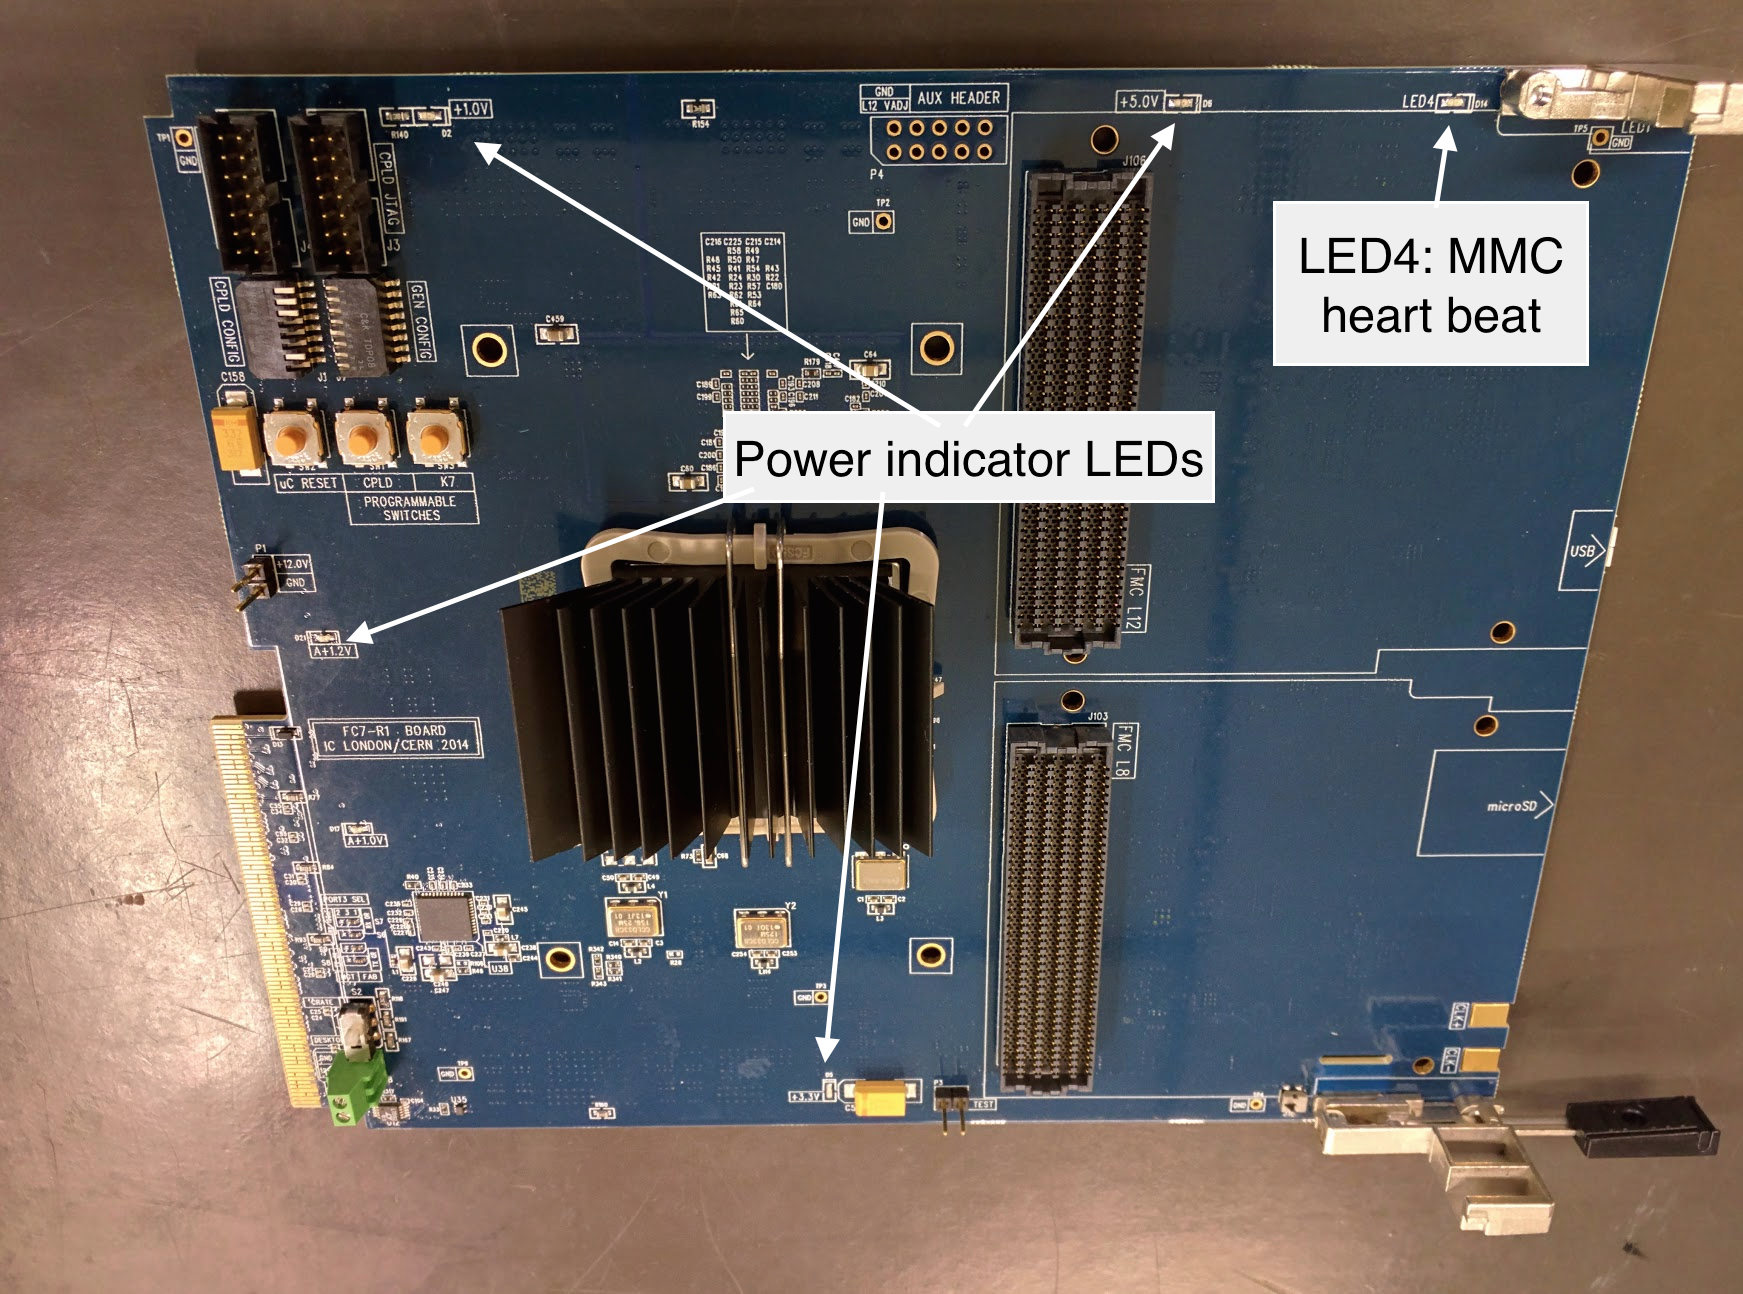
\includegraphics[width=\textwidth]{../images/FC7_side.png}
\caption[Side-view of the FC7 board]{\label{pic:FC7side} \textbf{Side-view of the FC7 board}\\
}
\end{figure}



\item[FC7 - front panel]\hfill\\
The FC7 is equipped with six LEDs on the front panel.
 Four of those LEDs have a defined behaviour on all FC7 cards.
 The remaining two LEDs are user defined and specific to whether the FC7 is configured as pixFED, pixFEC or tkFEC.
 The nameing convention of the LEDs can be found in figure \ref{pic:FC7front}.
 The purpose of the four standard LEDs can be seen seen in figure \ref{pic:LEDtable}.
 For the different flavours of FC7 cards in the Pixel DAQ system, the purpose of the user defined LEDs is summarized in table \ref{tab:UserLEDs}.


\begin{figure}[hf]
\centering
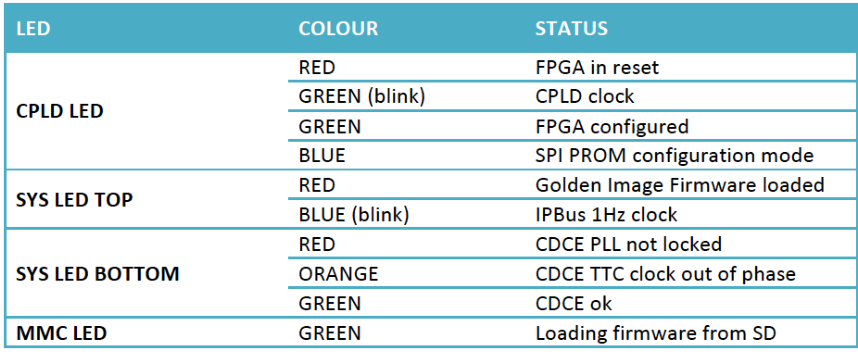
\includegraphics[width=\textwidth]{../images/LEDtable.pdf}
\caption[Purpose of the 4 standard LEDs on the FC7 front panel]{\label{pic:LEDtable} \textbf{Purpose of the 4 standard LEDs on the FC7 front panel}\\
}
\end{figure}


\begin{figure}[hf]
\centering
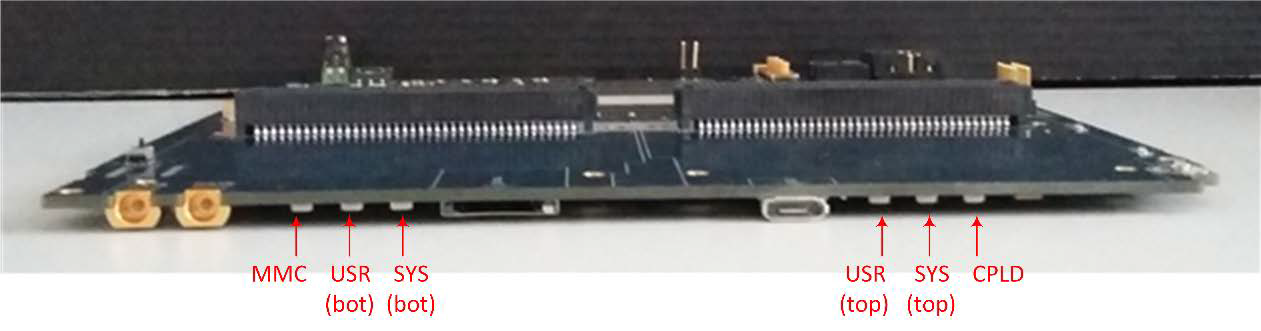
\includegraphics[width=\textwidth]{../images/FC7_front.png}
\caption[Front-view of the FC7 board]{\label{pic:FC7front} \textbf{Front-view of the FC7 board}\\
}
\end{figure}

\begin{table}
\begin{center}  
   \caption[User defined LEDs on FC7 front panel]{ \textbf{User defined LEDs on FC7 front panel} \label{tab:UserLEDs}}
        \begin{tabular}{c c c}
FC7 flavour & TOP User LED & BOTTOM User LED \\ \hline \hline
pixFED & unused & toggles with L1A triggers\\
pixFEC & PLL locked & unused\\
tkFEC & unknown & unknown\\
\hline
        \end{tabular} 
\end{center}
\end{table}                







\end{description}


\begin{figure}
\centering
\begin{subfigure}[t]{0.45\textwidth}
\centering
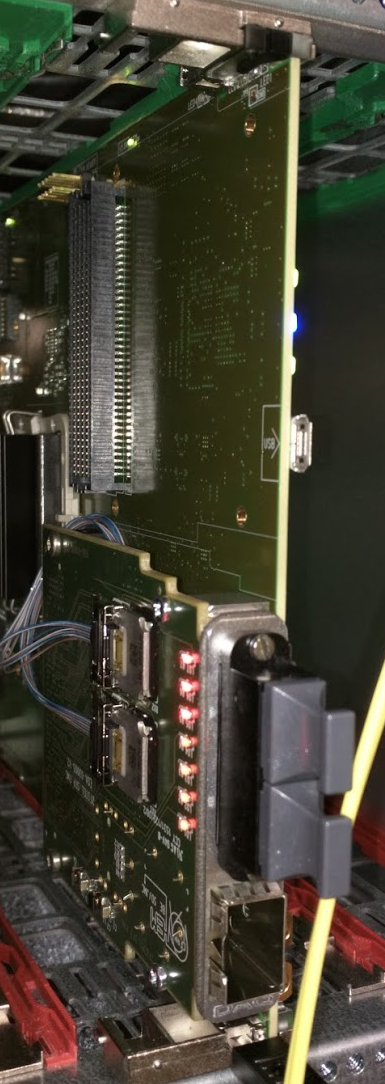
\includegraphics[width=0.75\textwidth]{../images/FED_FMC.png}
\caption[]{\label{pic:PLTTrackOcc_full}}
\end{subfigure}
\hfill
\begin{subfigure}[t]{0.45\textwidth}
\centering
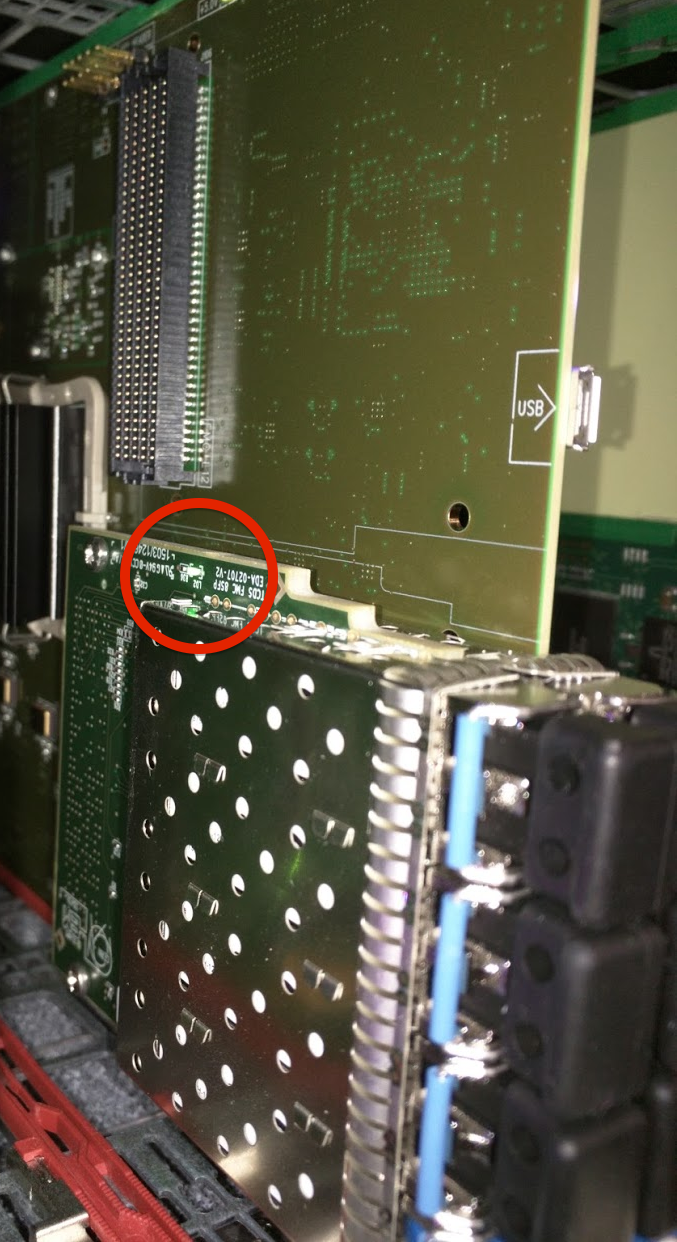
\includegraphics[width=0.75\textwidth]{../images/FEC_FMC.png}
\caption[]{\label{pic:PLTTrackOcc_cut}}
\end{subfigure}
\caption[Track occupancy for a single small angle telescope of the PLT]{\label{pic:PLTTrackOcc}
}
\end{figure}









% ******************************************************************************
\ifx\isEmbedded\undefined
\input{../biblio.tex}
\end{document}
\else
\fi
